\documentclass[UTF8,a4paper,fontset=none,zihao=-4]{ctexart}
\usepackage{fontspec}
\setmainfont{Times New Roman}
\setsansfont{Arial}
\setmonofont{Consolas}[Scale=0.85]
\setCJKmainfont{SimSun}[BoldFont=SimHei]
\setCJKsansfont{SimHei}
\setCJKmonofont{SimSun}
\usepackage[left=24mm,right=24mm,top=23mm,bottom=24mm]{geometry}
\usepackage{setspace,amsmath,amssymb,booktabs,tabularx,longtable,array,graphicx,xcolor}
\usepackage{tikz}
\usetikzlibrary{arrows.meta,positioning,fit,backgrounds}
\usepackage[most]{tcolorbox}
\usepackage[numbers,sort&compress]{natbib}
\usepackage{enumitem,fancyhdr,hyperref,caption}
\definecolor{ink}{HTML}{17324D}
\definecolor{teal}{HTML}{137D78}
\definecolor{light}{HTML}{EFF5F7}
\hypersetup{colorlinks=true,linkcolor=ink,citecolor=teal,urlcolor=teal,pdftitle={机器人自改进研究：完整对照结果与方向判断},pdfauthor={研究工作说明}}
\setstretch{1.18}
\setcounter{tocdepth}{1}
\setlength{\parskip}{0.28em}
\setlength{\emergencystretch}{2em}
\setlist[itemize]{nosep,leftmargin=2em,topsep=0.3em}
\setlist[enumerate]{nosep,leftmargin=2em,topsep=0.3em}
\ctexset{section={format=\large\bfseries\color{ink}},subsection={format=\normalsize\bfseries\color{ink}}}
\captionsetup{font=small,labelfont=bf}
\pagestyle{fancy}\fancyhf{}\fancyhead[L]{\small 机器人自改进研究说明}\fancyhead[R]{\small 2026年11月2日完整结果}\fancyfoot[C]{\thepage}
\setlength{\headheight}{16pt}
\newcolumntype{Y}{>{\raggedright\arraybackslash}X}
\newtcolorbox{keybox}[1][]{colback=light,colframe=teal,boxrule=0.6pt,arc=1.5mm,left=2mm,right=2mm,top=1.5mm,bottom=1.5mm,#1}
\newcommand{\ev}[1]{\textcolor{teal}{\small[#1]}}
\newcommand{\unknown}{\texttt{null}（未知）}
\begin{document}
\begin{center}
{\LARGE\bfseries\color{ink}机器人自改进研究\\[0.3em]完整对照结果与方向判断}\\[0.7em]
{\large 给导师的详细研究说明}\\[0.4em]
2026年11月2日\quad 本地仿真研究快照
\end{center}
\vspace{0.7em}
\begin{keybox}[title=先说当前判断]
有限对照已经做完。当前两个全局head候选都不采用，也不再加步数、扫系数或投入多卡。补入保留状态减轻了部分损害，却没有带来Long的520步新增能力。研究问题还值得有条件地转向，但目前没有已成立的方法创新或RSI证据。下一步只考虑一个尚未注册的前置诊断：学生能否在原联合指令下，接着老师的真实前缀完成任务。
\end{keybox}
\textbf{这份说明回答四件事。}我们想解决什么；系统现在到底学了什么；完整实验有什么收益和失败；哪些结果会改变接下来的研究决定。已完成结果、机制诊断与未注册提案分开写。

\textbf{已经闭合的关键证据：}
\begin{itemize}
\item 新比较库1197个完整模拟回合；其中Long为10任务、90条件、7策略，共630回合。520步parent为7/90，选择器6/90：修复0，伤害1。520/900端点，6个候选在parent失败的83条件上都失败。
\item 新source诊断选择器23/27，修复3、伤害1，但二值结果与固定候选完全相同。尚未证明按情境选择有额外价值。
\item 固定特权老师在4目标条件上520步为2/4、900步3/4；三个20步学生均未完成这些训练/目标条件。更强的全示范2000步BC出现少量完整行为，但520步目标0/4，并损害3个source条件。
\item 最新两臂各2000步和全部48回合已闭合。旧A八条件：parent8/8、原A保留6/8、补入保留7/8；source四条件：4/4、3/4、4/4；Long四条件520步均0/4。900步仅原A臂有1个第720步的晚成功。
\end{itemize}
\textbf{这次没有用工程修复冒充收益。}同进程第二次模型构造触发命名空间保护，属于基础设施故障。保留已完成首臂，在新进程只补原定第二臂；旧失败owner与全部费用仍保留。恢复没有改变原注册科学目标、数据、随机种子或末checkpoint。

\textbf{当前边界。}全部48例已经过独立原始/哈希/初态/成本和固定关键帧审查；没有运行中的实验。讨论中的24回合后缀诊断仅是未注册提案，查询预算尚未冻结，不能直接执行，也不计入已完成数据。

\textbf{阅读提示：}第1--3节讲问题和实现；第4--9节讲历史与完整对照；第10--12节讲成本、文献和下一步；末尾列可核查证据。全部机器人执行均为MuJoCo仿真，没有实机实验。旧版本保留。
\newpage
\tableofcontents
\vspace{1em}
\subsection*{本文常用词}
\noindent\begin{tabularx}{\textwidth}{p{23mm}Y}
\toprule
词语 & 本文的含义\\\midrule
parent & 本轮比较的共同起点策略，不表示它已掌握所有目标任务。\\
条件 & 任务、扰动、保存初态和执行噪声种子的组合；不是一个独立任务。\\
候选 & 从固定训练流程得到的策略版本。B选择器只在已有候选与parent之间选择。\\
修复/伤害 & 同条件下，parent失败而候选成功／parent成功而候选失败。\\
source/Long & 前者是原source任务划分；后者是LIBERO-Pro长任务块。两者不能混报。\\
BC/老师 & BC是模仿动作的学生训练；老师可有特权信息或手工控制，能力不能算到学生头上。\\
\bottomrule
\end{tabularx}
\newpage
\section{目标：让机器人改进策略，也避免把原本会的弄坏}
\subsection{研究问题为何重要}
长任务通常包含多个物体交互与连续阶段。机器人可能会抓一个物体，却在换目标、返回合适姿态或衔接下一段动作时失败。继续训练有时能补上失败，也可能破坏已有能力。只看平均成功率，容易把这些变化混在一起。

我们最初希望系统能先产生若干策略更新，再预测每个更新在当前情境下相对parent的收益，决定是否采用。进一步的目标是：系统根据真实修复反馈，学会下一轮怎样产生更有用的新修复，而不是一直沿用人工固定的训练规则。

这个方向的价值在于减少无效试错，同时控制伤害和测试开销。但价值必须体现在实际生成的策略上。一个分数更准的预测器、一个好看的流程图，或者一次辅助老师的成功，都不能代替闭环任务收益。
\subsection{用配对结果定义收益}
对同一个条件$c$，记完整任务成功为$Y(\pi,c)\in\{0,1\}$。本文使用
\[
 r(c)=\mathbb{1}[Y(\pi_{\rm parent},c)=0,\,Y(\pi_{\rm new},c)=1],\qquad
 h(c)=\mathbb{1}[Y(\pi_{\rm parent},c)=1,\,Y(\pi_{\rm new},c)=0].
\]
$r$是修复，$h$是伤害。在同一组条件、同一权重下，成功数变化等于修复数减伤害数。不同测试面板不能事后随意加权，拼成一个有利的“净收益”。例如，目标修好2个而source弄坏1个，应该先分别报告。

配对依靠相同的保存初态、环境资产、初始传感器和执行噪声设置。不同策略的动作分布会不同，后续轨迹不要求相同。条件之间仍可能共享任务与物体，不能把大量动作步或重复策略执行当成独立样本。
\subsection{当前真正要分开的四个问题}
第一，旧候选里有没有能修好失败的策略？第二，有外部帮助时，这个恢复能否执行？第三，受限制的学生能否从这些示范学会？第四，过去的更新反馈能否改善下一次新修复的产生方式？这四个问题的答案不必相同。现有证据主要涉及前三个；第四个还缺具体方法与决定性证据。

本研究使用本地DMPEL检查点与LIBERO/\allowbreak LIBERO-Pro资产\citep{dmpel,libero,liberopro}。它是有限的本地验证，既不是DMPEL整篇方法的复现，也不是完整benchmark或实机部署结论。
\section{当前系统怎么工作}
\subsection{策略看到什么，输出什么}
策略以两路RGB图像、7维关节位置、2维夹爪位置及语言指令为输入。视觉、语言和本体状态形成冻结空间特征，再经时序模块汇总，再由策略头输出7维动作的高斯混合分布（5个混合分量）。动作按已固定的执行规则采样；记录动作提议、对数概率、传感器和环境结果。

本地运行端口对摄像头、输入格式、动作节奏、精度和历史队列做过核对。这些工作保证比较可执行，但端口修复与数值一致性只是工程证据，不能算学到新任务。起点是作者source90预训练检查点，不代表完整适应Long任务后的系统。缺少目标域适应，本身就可能造成低成功率。
\par
\begin{figure}[htbp]
\centering
\begin{tikzpicture}[node distance=7mm and 7mm,>=Latex,box/.style={draw=ink,rounded corners,fill=light,align=center,text width=30mm,minimum height=13mm,font=\small},arr/.style={->,thick,draw=teal}]
\node[box](input){图像、关节、夹爪\\与语言};
\node[box,right=of input](policy){冻结主干\\加可训练适配器};
\node[box,right=of policy](gmm){高斯混合动作头\\按固定规则采样};
\node[box,right=of gmm](sim){MuJoCo执行\\完整任务反馈};
\draw[arr](input)--(policy);\draw[arr](policy)--(gmm);\draw[arr](gmm)--(sim);
\node[box,below=12mm of policy,text width=39mm](upd){人工固定的RL或BC更新\\得到新策略版本};
\draw[arr](sim.south)|- (upd.east);\draw[arr](upd.north)--(policy.south);
\node[below=7mm of upd,font=\small,align=center,text width=123mm]{实线是已经实现的策略更新回路。任务、奖励和训练规则由人固定；\\没有一个已验证的模块在学习如何设计下一轮更新。};
\end{tikzpicture}
\caption{当前策略与更新回路。输入、动作和反馈都来自模拟执行，不是实机系统。}
\end{figure}
\par
\subsection{候选策略如何产生}
原source训练包含3个训练种子和3轮更新，共288个在策略模拟回合、72个更新组。每组由当时的RL策略采集4个回合，再更新RL分支和共享数据BC分支。下一组继承各自上一组权重，所以确实是持续策略更新，而非每轮随机重训。

RL使用完整任务二值成功奖励和实际行为策略的动作密度；\textbf{不是用谓词阶段进度塑形奖励}。每组用其余轨迹的回报均值作为leave-one-out基线，采用PPO式裁剪替代目标，并加当前策略与参考策略的joint KL约束。这里保留混合分量索引作为辅助变量，joint KL是边际动作KL的上界，不能冒称精确计算了高斯混合边际KL。BC从同批RL采集中成功回合的动作做监督学习，不额外采集自己的经验。成功筛选本身也是该固定配方的一部分。共享数据可减少“是不是只因为多拿了数据”的混淆，但不意味着两个优化目标或有效监督完全等价。最终3个RL候选、3个BC候选用于后续固定比较。

训练信号审查发现288回合中265成功；72个四回合组有53组全成功、19组回报混合。实际RL优化126步，其中88步来自等回报组，38步有任务回报差异；BC共144步。当前四轨迹leave-one-out二值优势估计下，等回报组的任务优势为0，但KL仍可能造成更新，不能说所有RL都没有信号。共享数据也不表示实际优化步数或算力严格相同，因此原比较不是严格等算力的因果隔离。\ev{E12}

训练过程的任务选择、奖励、优化规则和轮数是固定的。即使某个版本比parent更好，也首先是这个固定流程产生了策略收益；不能直接升级为改进器学会了改进自身。
\subsection{B选择器学的是什么}
B不是动作控制器，而是部署前的候选收益预测器。它把初始情境、候选权重变化摘要、以及候选与parent的动作分布变化作为特征，估计完整任务成功的变化。标签来自已执行的parent/候选配对任务结果。

当前实现使用99维输入：3072维冻结情境特征经source拟合的PCA降到8维；54维修复描述经固定投影得到16维；动作分布差异有75维，包括均值、尺度及混合权重变化。后者需要查询候选策略头，因此即使不执行任务动作，也有模型查询成本。

预测器是由5个任务自助采样成员组成的小MLP集成。每个成员使用两层32宽隐藏层；另有共享parent预测分支。相对模型拟合$Y_{\rm candidate}-Y_{\rm parent}$；绝对模型及等价损失对照用于检查收益是否真的来自“相对建模”。不能仅凭改写标签就宣称方法新颖。

部署时，选择器取预测平均收益最大的候选；如果最大值不超过阈值，则回退parent；相近并列用固定字典序。集成标准差虽被记录，\textbf{当前选择规则并没有把它当统计置信保证}。阈值从固定集合$\{0,0.05,0.1,1\}$经校准选择；完整relative-joint主模型的新旧阈值最终均为0.05。
\section{为什么当前尚未验证RSI}
本文采用一个可测试的工作区分，不把它当作领域唯一正式定义：\textbf{策略更新}是策略参数改变后表现变化；\textbf{学习改进方式}则要求过去的修复反馈改变后来怎样产生更新，并让新生成的更新更有效。更强的递归主张还要证明改进后的改进器，能更好地修改改进方式本身。

当前已经实现前一种回路。B只给已有候选打分，没有决定下一轮用什么数据、目标或更新方式产生更好的新策略。多轮训练和权重继承不能单独补上这个缺口。系统也不必任意修改源码才可研究自改进；关键是明确学习对象和干预证据，而不是术语。

例如，若真反馈与打乱反馈对后来生成的策略没有不同影响，就不能把效果归因于学习修复反馈。若强固定BC在同样预算下已做到同样好，就没有证明学习改进器在这个问题上的必要性。把这些对照做出来是研究规范，\textbf{对照设计本身也不是新算法贡献}。

\section{实验谱系与新比较库协议}
\subsection{先分清几组数据}
\par
\begin{table}[htbp]\centering\small
\noindent\begin{tabularx}{\textwidth}{p{27mm}p{30mm}Y}
\toprule
数据块 & 数量与范围 & 用途和边界\\\midrule
原source训练 & 288模拟回合 & 产生RL及共享数据BC候选；不是独立测试。\\
旧配对库 & 912回合 & 48个source条件，parent与18个种子/轮次候选；不是Long结果。\\
新校准块 & 54条件$\times7=378$ & 仅用known候选标签选择阈值；不能据此报泛化。\\
新source诊断 & 27条件$\times7=189$ & 9任务，每任务3初态；已公开分析。\\
新Long块 & 90条件$\times7=630$ & 10任务，3扰动，3初态；主结果520步。\\
后续开发试验 & 截止闭合账140回合 & 含语言、归位、老师和学生等诊断；与benchmark库分列。\\
\bottomrule
\end{tabularx}
\caption{主要数据的用途。378+189+630=1197；截至最新完整审查的主线共2537行模拟试验，不是2537个独立任务。未注册的后缀提案不加入此数。}
\end{table}
\par
旧库为12个source任务、每任务2个初态与2个噪声种子构成的48条件，比较19个策略版本：$48\times19=912$。新库另放独立目录，不能把新1197追加到旧912后仍称同一个预先固定测试。两库任务、初态及候选范围不同，收益不能直接合并作一个主要检验；旧parent40/48与Long7/90也不能当成同一分布上的前后收益。旧912保留了39条数值失稳，新1197实际为0，不能混为一个失稳数。
\subsection{校准、诊断和Long怎么隔离}
校准沿用source划分中的9个任务，使用初态7、8、9、30、31、32，共54条件。新source诊断为另9任务的初态7、8、9，共27条件。Long为10任务，original、object swap、task perturbation三类，初态10、11、12，共90条件；执行噪声种子固定为20265100。

先对全部171个条件取得初始观测，并查询7个策略头，不执行受控任务动作。分数文件在任何新任务标签开放前保存。随后采集校准；再把诊断和Long的所有决策写入承诺文件；最后开放这些目标结果。
\par
\begin{figure}[htbp]\centering
\begin{tikzpicture}[>=Latex,node distance=6mm,box/.style={draw=ink,fill=light,rounded corners,align=center,text width=33mm,minimum height=17mm,font=\small}]
\node[box](a){171个初始观测\\7策略查询\\先保存预测};
\node[box,right=of a](b){采集54校准条件\\仅known标签\\确定阈值};
\node[box,right=of b](c){保存全部目标选择\\不读目标标签\\固定分析实现};
\node[box,right=of c](d){27诊断+90Long\\收齐全部回合\\一次冻结分析};
\draw[->,thick,teal](a)--(b);\draw[->,thick,teal](b)--(c);\draw[->,thick,teal](c)--(d);
\end{tikzpicture}
\caption{新比较库的标签时间边界。初始模型查询和reset settling也计成本；“不读成功标签”不等于没有模型调用。}
\end{figure}
\par
known指训练种子77210/77211的final候选；cold指77212。cold不进入B拟合、PCA或新阈值校准，但可作为保管方完整比较库中的控制策略。它是\textbf{候选种子的冷启动}，不是未见任务或预训练未见的证明。known/cold/all三个选择范围均固定后评估。
\subsection{时间端点和统计单位}
所有Long主结果统一为520控制步内完成完整任务。900步是同一条轨迹的延长，400步是敏感性分析；三者不能当成三批新样本。任务成功依原生完整谓词和数值稳定规则，阶段谓词只作诊断，不能代替主成功。

冻结分析包括四项任务簇配对符号翻转检验，并做Holm校正：Long新校准选择器对parent；Long新阈值对旧阈值；source诊断新选择器对parent；Long三RL均值对三共享数据BC均值。Long按10任务簇，source诊断按9任务簇，不按630条执行记录独立检验。

在完整库结束前曾公开Long前7个任务簇的探索读数，完整结果因此不能包装为从未看过的确认。该中期暴露没有用于改动冻结采集方案，但必须披露；之后也不能用这批标签调参再称独立验证。
\section{source证据：有策略收益，尚无选择器独特收益}
\subsection{旧912库应怎样解读}
旧48条件上，parent为40/48；final三RL分别45、42、40，三共享数据BC为44、43、42。最好的RL有5次修复、0次伤害；其他种子可能同时修好与破坏条件。这说明固定训练有局部策略收益，也说明种子和训练方式差异不能省略。
\par
\begin{table}[htbp]\centering\small
\begin{tabular}{lrrr}\toprule
旧48条件上的final策略 & 成功 & 修复 & 伤害\\\midrule
Parent &40&--&--\\
RL 77210 / 77211 / 77212 &45 / 42 / 40&5 / 4 / 1&0 / 2 / 1\\
共享数据BC 77210 / 77211 / 77212 &44 / 43 / 42&5 / 4 / 3&1 / 1 / 1\\\bottomrule
\end{tabular}
\caption{旧source库的final候选。分母均为48条件，不是Long90。该表不是事前选定最佳种子后的确认收益。}
\end{table}
\par
旧B主要比较未表现出相对收益模型的泛化优势。原3项主要检验最终Holm校正$p$均为1。EVSI预算16的离线复用读数为85\%，随机83.75\%，差1.25个百分点，但只有2个诊断任务簇、8个条件。10次数值重复改变查询和后验随机性，不增加机器人任务证据。全部旧bank已经采集，不能据此声称实际省掉模拟回合或时间。

较早报告中的“多重比较等待active结果”是写文件时的中间状态；最终active汇总已完成，未使用缺失结果占位。本文引用最终汇总，而非把旧pending误写为未完成。\ev{E1--E2}
\subsection{新9任务诊断有什么变化}
新27条件上，parent为21/27；RL三种子23、22、23；BC为22、22、23。相对选择器known、cold、all的固定0、旧阈值、新校准读数均为23/27。相对all选择器有3次修复、1次伤害。

但是all选择器在21/27条件上选cold RL，其余6次切换后的二值结果仍与固定cold RL完全一致。\textbf{因此23/27不能证明情境选择比固定策略更有用。}完整relative-joint主模型的新旧阈值同为0.05，也没有证明本轮新校准带来收益。
\par
\begin{table}[htbp]\centering\small
\noindent\begin{tabularx}{\textwidth}{Yrrr}\toprule
新source27条件的规则 & 成功 & 修复 & 伤害\\\midrule
相对／独立绝对／等价绝对模型 &23&3&1\\
共享绝对模型 &22&2&1\\
仅情境／情境+权重摘要（去行为） &21&0&0\\
情境+行为（去权重）／情境+ID+行为 &22&2&1\\
去显式情境 &22&2&1\\
仅修复特征 &23&3&1\\
完整校准复测门控 &22&2&1\\
PACE适配（16/32/64/324标签） &21&0&0\\\bottomrule
\end{tabularx}
\caption{同一目标块的匹配控制与消融，均按520步、all候选范围。预测器用新校准阈值；完整复测和PACE按各自cal标签规则。PACE四预算为16/32/64/324个child标签。这些仅是本地适配，不是完整论文复现。}
\end{table}
\par
“去显式情境”仍保留依赖观测的动作分布特征，不能叫完全无情境控制。部分控制相近或更弱，也不能用来反推相对标签是新颖性来源。旧2任务诊断阴性和新9任务描述性收益范围不同，均保留，不择一讲述。
\section{Long证据：主要问题在当前候选没有新增覆盖}
\par
\begin{table}[htbp]\centering\small
\noindent\begin{tabularx}{\textwidth}{Yrrr}\toprule
Long90条件，520步主结果 & 成功 & 修复 & 伤害\\\midrule
Parent &7&--&--\\
RL三种子 &3 / 5 / 5&0 / 0 / 0&4 / 2 / 2\\
共享数据BC三种子 &5 / 6 / 7&0 / 0 / 0&2 / 1 / 0\\
相对／绝对／等价绝对选择器 &6&0&1\\
共享绝对模型 &5&0&2\\
仅情境／情境+权重摘要（去行为） &7&0&0\\
情境+行为（去权重）／情境+ID+行为 &6&0&1\\
去显式情境／仅修复特征 &5&0&2\\
完整校准复测门控 &5&0&2\\
PACE适配各预算 &7&0&0\\\bottomrule
\end{tabularx}
\caption{Long与source分开报告。候选顺序为77210、77211、77212。收益/伤害均相对同条件parent。}
\end{table}
\par
\subsection{为什么先不继续复杂化当前选择器}
在520/900步端点，parent失败的83个条件中，6个候选全部失败。包含parent的事后oracle也只有7/90，事后最佳固定BC同为7/90。all/cold范围选择器为6/90，known范围为5/90；all选择器离这个有限库上界差1次。oracle只是看到全部标签后的描述工具，不是可部署方法。

这并不证明“修复生成不可能”，而是证明\textbf{本次测到的固定库没有补充这些失败条件的成功}。继续调一个更复杂的路由器，最多恢复这个库已有的覆盖，不能产生库外能力。相比之下，怎样生成学生真能学会的新行为，更值得先查清。
\subsection{统计结果支持什么}
\par
\begin{table}[htbp]\centering\small
\noindent\begin{tabularx}{\textwidth}{Yp{22mm}p{34mm}r}\toprule
冻结主要比较 & 差值（百分点）& 任务簇95\%区间 & Holm $p$\\\midrule
Long：新选择器$-$parent & $-1.11$ & $[-3.33,0]$ &1\\
Long：新阈值$-$旧阈值 &0&$[0,0]$&1\\
source诊断：新选择器$-$parent &$+7.41$&$[-7.41,25.93]$&1\\
Long：三RL均值$-$三BC均值 &$-1.85$&$[-4.81,0]$&1\\\bottomrule
\end{tabularx}
\caption{效应量和任务簇bootstrap区间与冻结分析对账。少量任务簇下，区间和检验精度有限。}
\end{table}
\par
校正$p=1$不是等效性证明，也不是所有未来方法都无效的结论。它意味着这些主要比较没有给出预定意义上的改善证据。新旧阈值完全相同时，零差值也不能推广成两类校准方法处处等价。

520与900步下parent均7/90，选择器均6/90，修复0、伤害1。400步下parent6/90，选择器6/90，修复1、伤害1；这说明端点会改变配对解释，因此不能事后挑400步当主结果。
\subsection{失败不都等于“交接坏了”}
\par
\begin{figure}[htbp]\centering
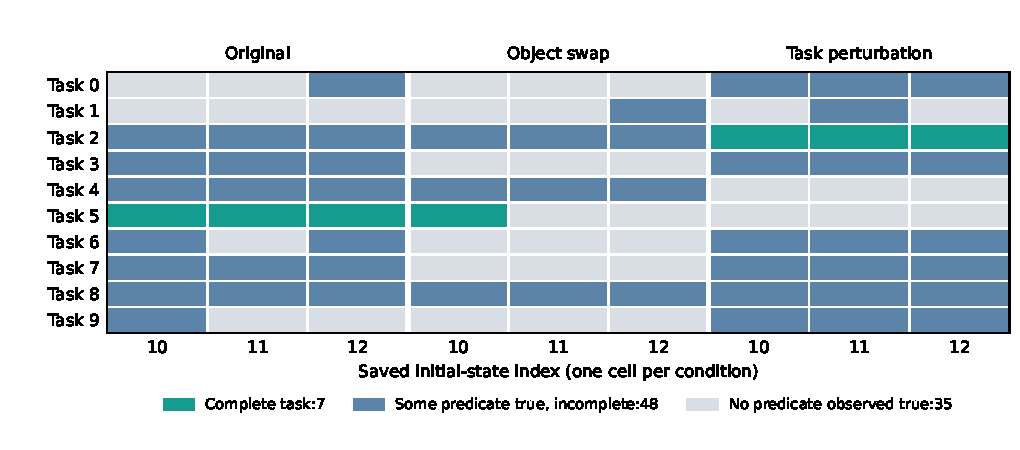
\includegraphics[width=\textwidth]{images/parent_Long90.pdf}
\caption{原parent90个Long条件在520步内的真实描述图：7个完整成功、48个曾出现部分谓词为真但未完成、35个未观察到谓词为真。每格一个条件。原始初始truth未另存，不能把48格都解释为新学会第一阶段或交接失败。}
\end{figure}
\par

原parent90条件中，7个完成完整任务；35个在已记录的动作后状态里没有任何目标谓词为真；48个曾有部分谓词为真但没完成。原轨迹未另存初始谓词真值，任务定义中的谓词顺序也不代表技能执行时序。

因此不能把48个全叫“已经完成第一技能、只差handoff”。其中可能有初始状态已满足某谓词，也可能是不同目标或后续退化。两任务的归位诊断不能解释所有83个失败。检查点适用域、任务语言、动作/夹爪执行及原子行为覆盖，仍是不同候选解释。\ev{E3,E7}
\section{从辅助老师到学生：有执行能力，不代表已经学会}
\subsection{辅助流程做了什么}
开发诊断集中在两个把两个物体放入篮子的Long任务。固定流程先使用第一段指令；当原生第一目标谓词变真时，由GT触发阶段切换，再执行60步手工返回动作、保持夹爪打开，之后使用第二段指令继续。这不是学生自己的恢复决策。

原4个开发条件上，拆句但不归位为0/4；只降低正常采样尺度仍0/4；归位并用原learned采样尺度在520/900步均为4/4；归位加低尺度在520步2/4、900步3/4。归位改变姿态、等待时间、夹爪、历史队列和随机数消耗等多个因素，不能将收益唯一归因于末端位姿。

换到4个目标条件，固定老师在520步为2/4，900步为3/4。一个案例在第623步才完成，另一个没完成第一目标，根本没触发归位。这里初态与执行噪声同时变化，不是纯初态因果试验。所有老师结果都与学生分列。
\subsection{学生具体学了什么}
从原开发条件的7条成功老师轨迹取得3163个动作。7条并不代表7个独立任务，它们只覆盖4个相关条件、2个任务。重放时用\textbf{原联合指令}缓存冻结空间特征（包含视觉、语言和本体状态），让训练输入尽量接近学生部署；动作目标仍来自带特权辅助的老师。

最初两个学生均使用128个老师动作目标、128个保留目标；一个均匀采样，一个从局部恢复窗口采样。每步呈现16个老师目标和16个保留目标，共20步。训练6个时序注意力适配器，总73728参数；损失为动作负对数似然加$0.001$倍joint KL，参考为共同parent。只评估最后一步，不挑最优检查点。

第三个学生保持均匀目标、采样序列、损失与20步预算，把可训练部分移到策略头第一共享层，使用rank72、alpha144的适配器，同样73728参数。它同时改变位置、秩和优化几何，不能称纯层位置消融或等FLOPs比较。8个零B查询的一致性核对只证明初始化可比，不是任务收益。
\par
\begin{table}[htbp]\centering\small
\noindent\begin{tabularx}{\textwidth}{Yrrr}\toprule
策略 & 原老师训练条件 & 目标条件 & source保留条件\\\midrule
Parent &0/4&0/4&3/4\\
均匀时序BC（20步） &0/4&0/4&4/4\\
局部时序BC（20步） &0/4&0/4&3/4\\
均匀head BC（20步） &0/4&0/4&3/4\\
固定特权老师 &4/4$^{*}$&2/4（520）&不作此比较\\\bottomrule
\end{tabularx}
\caption{三个学生的520/900完整成功数相同。$^{*}$原老师4/4指原归位learned分支在520/900步均4/4；目标老师900步为3/4。source仅4条件、2任务，不能代表完整旧能力。}
\end{table}
\par
均匀时序BC在source修复1、伤害0；局部BC修复1、伤害1，成功总数仍3/4；head BC修复0、伤害0。局部窗口没有优于均匀配方。实际每条老师轨迹的配额和呈现已核对，早先怀疑的配额不匹配没有发生，不能再作为解释。
\subsection{拟合诊断说明了什么，没说明什么}
在真正被训练呈现过的servo目标上，均匀学生19个目标的归一化动作空间的oracle最近混合均值L2距离为$0.4565\to0.4485$，局部学生32个目标为$0.4448\to0.4343$。这两个目标集不同，不能直接作总体性能排名。

在全部420个servo动作上，head学生NLL为$33.0007\to12.9653$，但oracle最近均值距离仅$0.427685\to0.421922$，平均normal sigma从0.075046变为0.084626。NLL降低可能伴随多个分布参数变化；oracle最近分量也不一定是实际采样分量。

这些都是描述，不证明已经充分拟合，也不证明sigma变化是失败唯一原因。三个有限配方失败不能排除BC，更不能据此认定某个梯度通路必然被阻断。监督覆盖、目标损失、表示、优化预算及闭环偏移都尚未被唯一隔离。\ev{E4--E6}
\section{完整的强固定BC结果：能偶尔完成，但不能采用}
\subsection{比20步配方强在哪里}
这轮使用全部7条旧老师轨迹的3163个动作，加原128个保留动作目标。从原作者$\pi_0$与新零B head开始，\textbf{不是从20步学生继续}。head结构、学习率和损失不变，固定2000步，每步16老师、16保留，共64000次loss呈现、128000次当前/参考分布前向。63个早期目标也进入训练，使用真实长度1--10的动作前历史，不做假填充。

与20步均匀head相比，老师池从128到3163，更新数增加100倍，短历史覆盖和按动作均匀采样的权重也改变。因此，结果只能归于这个更强的固定监督配方，不能归因某一个因素，更不能当同预算新方法优势。四个旧参考actor的结果直接复用，没有重复执行。
\subsection{12回合完整结果与三个成功发生的时间}
评估为原4训练条件、4目标条件、4个source条件。全程使用原联合指令，无GT控制、无手工归位。结果、视频、初始观测、事件、参数和冻结分析均已完成独立对账；72个选定原始关键帧已目视。这不是逐帧播放审查，也不是实机验证。
\par
\begin{table}[htbp]\centering\small
\begin{tabularx}{\textwidth}{Yrrr}\toprule
条件组与端点 & Parent & 全示范head BC & 修复 / 伤害\\\midrule
原训练条件，520步 &0/4&1/4&1 / 0\\
原训练条件，900步 &0/4&2/4&2 / 0\\
目标条件，520步 &0/4&0/4&0 / 0\\
目标条件，900步 &0/4&1/4&1 / 0\\
Source保留检查，520步 &3/4&0/4&0 / 3\\
Source保留检查，900步 &3/4&0/4&0 / 3\\\bottomrule
\end{tabularx}
\caption{固定2000步BC的完整描述结果。每组4条件；逐步动作和复用旧结果不能算新增独立样本。900是同一轨迹延长；后续新保留状态对照将source上限固定为520。}
\end{table}
\par
三个完整成功分别发生在第372、531和694步：前两个属于原训练条件，第三个属于目标条件。因而只有372步成功进入520主端点。694步正例说明这个学生在某个已知任务条件下确实完成过，但不能替代主端点的0/4目标结果。不能只展示该视频而略掉3次source伤害。

\begin{keybox}[title=这一轮改变了什么判断]
“学生完全学不到完整行为”已经过强，应撤下。更准确的判断是：更充分的普通监督训练能产生少量完整行为，但当前配方没有达到目标520步收益，并破坏了3个原本成功的source条件。拒绝这个候选，不继续靠增加选择器复杂度来包装它。
\end{keybox}
\subsection{离线拟合改善不等于闭环修复}
在全部3163个老师动作上，动作NLL从parent的$-14.4284$变为$-22.5441$，oracle最近混合均值L2从0.14159变为0.12676。在420个servo目标上，NLL从33.0007变为$-15.6069$，最近均值L2从0.42768变为0.37490，平均normal sigma从0.07505变为0.11610。这里L2是7维归一化动作空间距离，不是米；连续密度的NLL可以为负。

这些变化表明动作拟合确实改变，却没有保证目标条件的520步完成。oracle最近分量不等于实际采样分量；更高的sigma也不能被直接认定为失败原因。没有事前的充分拟合阈值，2000步不是已证明的监督上限。新head只做3291次离线密度前向，旧四actor的13164条打分直接复用；没有把离线打分当新回合。
\subsection{为什么不能直接说“旧能力全部遗忘”}
128个保留动作来自同一\texttt{libero\_90}任务空间中的8、13、29、35、48、67、86、87号任务；这次source保留检查来自9、34号任务。两边有场景、物体和技能重叠，但不是相同任务或相同行为状态支持。原128个动作来自多轮RL行为策略采集的成功轨迹，\textbf{不是parent示范}；parent只作为共同KL参考。

因此，9/34上相对parent的3次伤害是确定的配对记录，却不能外推为原A八任务全部遗忘。保留动作拟合好，也不证明已经保住9/34的闭环能力。需要区分任务与行为状态支持、保留目标本身以及模型更新的影响。因此随后开展同预算、统一保留目标的普通对照，见下一节；没有先发明学习路由。\ev{E13}
\section{保留状态对照完整结果：损害减少，但目标能力没有增加}
\subsection{这次只改变什么}
两臂都是普通BC。原A臂保留原128个A状态；补入臂保留其中64个，再加既有source任务9/34、初态7/8四条head20轨迹各16个状态，共128个。四条均纳入，包括失败轨迹，不按成功筛选。它们是head20访问的状态，不是parent的真实访问分布。

两臂都去掉保留动作NLL，只在保留状态上蒸馏同一parent分布。老师动作监督不变。每步16老师目标、16保留状态，实际目标为
\[
\frac{1}{32}\sum_{i=1}^{16}\bigl[-\log\pi(a_i\mid x_i)+0.001D_{\rm joint}(\pi\Vert\pi_0;x_i)\bigr]
+\frac{1}{32}\sum_{j=1}^{16}D_{\rm joint}(\pi\Vert\pi_0;z_j).
\]
这里$D_{\rm joint}$是当前到parent的辅助分量joint KL上界，不是精确边际GMM KL。保留项系数固定1，不读取行为动作标签。两臂均从作者$\pi_0$和相同零B head开始，不续训另一臂或历史学生。

head rank72、alpha144，73728参数；lr$10^{-4}$、wd0、clip1，各2000步，只评估末checkpoint。训练采样种子20265500，两臂的teacher/retention索引序列一致。每臂完成32000个老师目标及32000个保留状态呈现，128000次当前/参考分布前向；两臂共4000步、128000次loss呈现、256000次前向。

老师池仍3163个动作，实际固定有放回序列覆盖3162种，其中一个目标0次；事前已记录，没有换seed或补抽。所有保留状态都有10个真实过去/当前特征，老师历史为真实1--10，不补帧、不用未来帧。原A64并非每任务均匀减半，任务67状态数从17降到4；这项潜在代价已经纳入全部旧A八任务的验收。
\subsection{16条件、48回合，主端点不变}
旧A八任务各初态20；source9/34各初态20/21，共4条件；Long0/7各初态20/21，共4条件。共16条件、12个已知任务，parent和两个候选各执行一次，合计48回合。执行种子20265510。source上限520，Long同轨迹最多900，统一以520为主端点。
\par
\begin{table}[htbp]\centering\small
\begin{tabularx}{\textwidth}{Yrrr}\toprule
条件组／端点 & Parent & 原A保留臂 & 补入保留臂\\\midrule
旧A，520步（8条件） &8/8&6/8&7/8\\
Source，520步（4条件） &4/4&3/4&4/4\\
Long，520步（4条件） &0/4&0/4&0/4\\
Long，900步同轨迹延长 &0/4&1/4&0/4\\\bottomrule
\end{tabularx}
\caption{完整冻结读数。原A保留臂为\texttt{oldA\_KL}，补入臂为\texttt{coverage\_KL}。旧A/source没有900步观察，值为null，不能填0。}
\end{table}
\par
\begin{table}[htbp]\centering\small
\begin{tabularx}{\textwidth}{Yrr}\toprule
相对同条件parent的修复／伤害 & 原A保留臂 & 补入保留臂\\\midrule
旧A，520步 &0 / 2&0 / 1\\
Source，520步 &0 / 1&0 / 0\\
Long，520步 &0 / 0&0 / 0\\
Long，900步延长 &1 / 0&0 / 0\\\bottomrule
\end{tabularx}
\caption{成功与伤害分组报告。Long的parent为0/4，没有伤害机会；0伤害不是安全或能力保留证据。}
\end{table}
\par
唯一Long晚成功是原A臂的任务7、初态21，第720步完成。它是真实正例，应保留；但不能替代520的0/4。补入臂相对原A臂在900又失去了这个成功，因此不能只展示source损害减少而忽略目标差别。
\subsection{本次支持什么解释}
补入臂相对原A臂挽回旧A任务13和source任务34/初态21。它在source保持4/4，是保住parent已经会的能力，不是新增修复，因为parent本来4/4。旧A仍损害任务67。\textbf{任务67两臂都失败，不能将它单独归因补入臂把该任务状态从17减到4。}

本次支持“保留状态集合会影响损害”的有限观察，不支持纯任务覆盖的单因素因果结论：任务与行为状态支持同时变，原A状态也减少。两臂均改了历史全示范BC的保留目标，因此不能将新结果与历史source3害作前后因果比较；初态和执行seed也不同。

所有比较只有一个训练种子与一个执行种子，条件共享任务。这里没有新增IID检验或显著性主张。16次初始化parity只证明起点与输出端口可比，不是16个任务收益；没有额外teacher采集也不等于训练或测试免费。
\begin{keybox}[title=这次门槛的决定]
拒绝当前两候选，停止扩大这套固定全局head配方，不再追加步数、扫描系数或组多卡。保留状态支持减轻了部分损害，却没有产生Long的520步新增能力。否定的是这两种已完成配方，不是全部BC、全部global-head结构或全部Long任务，更不是证明机器人无法学习恢复。
\end{keybox}
\subsection{基础设施恢复和证据完整性}
首臂完成2000步后，同一Python进程第二次构造native模型触发命名空间保护。第二臂当时step0、0前向、0查询。该故障不能当任务失败，也不能卸载模块绕过保护后盲重启。

恢复在独立进程只补原定第二臂。原per-arm训练块经AST逐项核对不变；共同初始全参数digest相同，两臂各自实际完成4个plain与4个零B查询。未冒称跨进程执行过原同进程\texttt{torch.equal}检查。两份真实收据由独立CPU聚合器合并，原失败owner没有被改写成成功；新增恢复owner的四个阶段才是成功闭合。

独立原始复核核对50150文件哈希、全部18069查询/事件/动作、三actor初态和原始完整成功；本轮无策略数值失败或物理数值失稳。全部48个MP4由CPU完整解码18117帧，即18069个post-action帧加48个初帧。root实际看完12张sheet中的288个固定帧位，共192个不同源位置；\textbf{不是人工逐帧看完18117帧}。

初态PNG保留原sensor RGB；MP4有压缩，不能要求它与原sensor逐像素相同。contact sheet的caption在原帧外，原256$\times$128帧像素未缩放。BDDL谓词顺序不是技能时序，选定关键帧也不能唯一解释失败原因。原结果、轨迹、视频、事件、失败日志和旧报告全部保留。\ev{E14--E17}
\section{成本和本地资产：什么已经花了，什么还不知道}
\subsection{方法访问成本与实际采集成本分开}
相对新校准按最小足够标签计划访问51个child与51个parent标签，共102；密集参考访问216个child与54个parent，共270。2936个工程用例与30次旧数据次级回放支持最小访问与完整校准严格选择等价；这不等于机器人收益或新颖性。

实际研究为了比较已经采齐378个校准回合，所以这次少读标签没有省掉任何实际回合。历史B还访问过480个child与40个parent标签。初始特征、候选头查询、reset settling和CPU预测准备均须收费；不能只留下102这个好看的数字。
\par
\begin{table}[htbp]\centering\small
\noindent\begin{tabularx}{\textwidth}{Yrp{45mm}}\toprule
数量 & 数值 & 范围解释\\\midrule
新比较库模拟回合 &1197&54校准+27诊断+90Long，各7策略\\
新库任务控制步 &671788&不含reset settling\\
新库reset settling &11970&与任务控制分列\\
初始full-policy / reference查询 &1197 /1197&171初态的预查询\\
bank内策略／额外参考头查询 &671788 /1197&与初始probe分开\\
初始探测settling &1710&另计\\
已闭合主线试验行 &2537&含最新48回合；不是独立任务\\
已闭合主线任务控制 / settling &1004079 /25370&含以往开发试验\\
HD/老师缓存重放 &21&另列，不是新策略结果\\\bottomrule
\end{tabularx}
\caption{已闭合成本。scope不同的行不能直接相加；未注册的后缀提案不计入2537。}
\end{table}
\par
已闭合主线为$288+912+1197+140=2537$。旧78次中断开销仍保留；其后完成的重跑已经在相应bank中，不能再次算成新增回合。基础设施删失不是任务失败；数值失稳按原规则保留，不能按结果挑掉。
\subsection{最新对照新增的真实费用}
本轮实际新增48个回合、18069个任务控制、480个settling，两次训练共4000优化步、128000目标/状态呈现、256000次分布前向。16次parity有编码/头查询/动作采样，但0物理控制；没有新增teacher采集，也没有新离线密度评分。累计开发140回合、6次开发训练；这不包括原source多轮训练的全部优化次数，也不是工作区所有历史运行的无范围总数。
\par
\begin{table}[htbp]\centering\small
\begin{tabularx}{\textwidth}{Yrp{52mm}}\toprule
时间边界 & 秒 & 怎么理解\\\midrule
原失败训练命令（含已完成首臂） &3183.9016433&原失败保留，不再加其中的训练loop\\
恢复owner观察区间 &7184.6742042&包含下面四个恢复phase\\
\quad{}剩余第二臂训练命令 &2679.8558042&与原失败命令是不重叠区间\\
\quad{}CPU双臂聚合命令 &255.1872155&只校验／复制／汇总，不是新训练\\
\quad{}48例评估命令 &4080.8377943&含推理、模拟、通信和写盘\\
\quad{}冻结分析命令 &146.2326172&一次完整分析，不新增任务样本\\
Root原始复核外部／内部 &175.8049008 /174.9946898&内部已含于外部，不相加\\
补充CPU审查 &2.1875372&独立记录，0模型／模拟\\
视频准备CPU管线wall &34.0871210&含解码与保存，非人工观看时长\\\bottomrule
\end{tabularx}
\caption{最新实际计时来自闭合JSON收据。所有嵌套计时不重复相加；human、审稿思考及全项目端到端墙钟仍为null。}
\end{table}
\par
评估query时间1638.4458秒、packet写盘982.3917秒已嵌套在逐回合wall3993.6598秒及评估外部命令中；视频解码wall16.6855秒也已含于34.0871秒准备管线。不能把这些内部项再叠加。原owner没有成功complete，原失败和恢复区间也不能伪装成一次无中断成功运行。\ev{E16--E17}
\subsection{时间与算力不能怎么报}
新库逐回合wall之和为93138.95秒，但它不是从训练到部署的项目端到端时间。较早20步head学生的12例评估外部命令耗时2151.05秒，其中推理约1033.39秒、packet写盘约577.00秒，其余包括启动、模拟、通信等。新库推理60713.19秒嵌套在回合wall内，B预测CPU准备约7.10秒另有边界。内部计时已经包含于外部，不能重复相加，也不能将余项全叫物理模拟。

较早全示范单臂2000步BC新增12个回合、9697个任务控制、120个settling；训练新增128000次分布前向，离线新增3291次密度前向，8次初始化工程查询为0物理控制。训练命令外部5497.10秒，评估2768.58秒，分析101.05秒，离线102.32秒；owner内部观察区间8475.56秒已包含各阶段，不能再相加。原20步head的owner与最初中断分析wall未完整闭合，整项目wall也未知，记为\unknown{}，不是0。等待中断的日历间隔也不能自动算GPU计算时间。

当前没有证据表明多卡能解决科学瓶颈。现管线有串行依赖，利用率单次采样不代表长期利用率；GPU分配器峰值也不等于整卡显存。先得到可重复收益或明确容量瓶颈，再按任务数、种子数、卡时提出扩展需求。\ev{E6,E10}
\subsection{手里有哪些可复查材料}
\noindent\begin{tabularx}{\textwidth}{p{31mm}Y}\toprule
资产类型 & 已保存内容与限制\\\midrule
source训练NPZ & 动作、冻结空间特征、行为log概率、机器人状态、奖励、子目标、warning、初始simstate；\textbf{不能说都有每步完整物理状态}。\\
配对/开发轨迹 & 逐步完整物理状态、动作、机器人与谓词事件、初始观测及哈希，可做严格重放核对。\\
模型和决策 & parent/候选权重、训练收据、B变换与分数、标签开放前保存的选择、冻结分析。\\
视频和材料 & 录制的真实仿真视频、严格状态重放的HD、图表和讲稿；不是实机录像。关键帧审查不等于逐帧完整播放。\\\bottomrule
\end{tabularx}
原开发与完整2000步BC各72个选定关键帧已分别审查；最新48例的288个固定帧位另有独立签收。关键帧不能证明释放后长时间稳定。完整汇报包保留原始与后续版本；媒体回放不会增加独立策略成功样本。
\section{相近工作已经做到哪里}
本文基于本地保存的原文与版本。只把明确核过的机制用于比较，不把已有概念换名当创新。9条参考文献见末尾，其中前3项提供策略与benchmark背景，后6项用于定位研究问题。
\par
\begin{table}[htbp]\centering\small
\noindent\begin{tabularx}{\textwidth}{p{30mm}Y}\toprule
工作 & 对本项目最直接的约束\\\midrule
DMPEL、LIBERO、LIBERO-Pro\citep{dmpel,libero,liberopro} & 本地checkpoint与任务资产来源；当前不是DMPEL完整专家库及整论文复现。\\
Physical RSI\citep{physical_rsi} & RSI讨论的背景。不能把某个操作性标准说成唯一正式定义。\\
LRS\citep{local_recovery} & 已用学生执行反馈决定恢复监督范围；“学生感知的恢复示范”不是空白。\\
CUPID\citep{cupid} & 已用任务表现估计示范价值；“挑更有用数据”不是天然新点。\\
PRACTICE\citep{practice} & 已从历史技能和新轨迹产生增、改、合并、删除编辑，并继续训练skill learner。\\
PBYM\citep{predict_before_modify} & 已根据过去修改的预测误差更新IDM，再用于后续修改预测与修订。\\
Recursia\citep{recursia} & 已研究共享执行栈、技能契约和handoff；拼技能和修交接不能直接宣称新颖。\\\bottomrule
\end{tabularx}
\end{table}
\par
\subsection{最强反方不是“没有人研究过自改进”}
PRACTICE和PBYM已覆盖泛泛的“过去反馈改善下一次修改”。我们的候选区别最多是连续控制策略的实际修复、旧能力伤害以及真实交互成本的隔离证据；这个场景区别本身还不是新方法。必须给出具体机制，并证明它优于兼容的强基线。

LRS使用学生执行决定监督长度，其teacher与固定配方仍应区分。CUPID官方所读实现使用$+1/-1$反馈，没有同批均值baseline；有限全失败组也可能产生非零估计，不能写“全失败必无信号”。它的投影4000、ridge0不能不检查秩就套到本地有限数据；任何投影、阻尼变化都须叫适配。

所读CUPID默认lowdim重训脚本是在新输出目录按种子从头训练筛选数据，不是从用于打分的策略继续20步。本地有限parent更新是另一个明示适配。我们也没有用老师servo动作伪造普通on-policy RL对照；两者指令和实际行为密度不相同。

文献核对提供研究边界，不等于复现了这些论文的机器人收益。部分新工作只有原文审查，没有拿到可审官方实现，不能冒称代码复现。\ev{E8}
\section{当前判断与验证优先级}
完整有限对照的判断已经签收：\textbf{当前两种全局head配方不采用、不扩大，不组多卡；保留研究问题，先过一次有限的后缀可恢复性门槛。}当前没有值得多卡放大的正方法。单卡已经完成规定训练与采集，没有证据表明多卡容量是科学瓶颈。
\subsection{为什么先不直接做闭环恢复数据训练}
一种初始意见是：按同teacher/采集预算，比较学生失败状态上的恢复监督与新完整老师示范。这是有意义的固定强基线，但不是创新，LRS与CUPID已经覆盖相邻问题。

另一意见更优先检查：学生究竟能不能从老师实际产生的状态继续完成。当前采用后者作为前置门槛，因为\textbf{现有GT/home/分段老师不等于任意学生偏离状态上都可靠的恢复oracle}。不能把尚不存在的恢复标签接口当作已准备好，更不能自动开展DAgger式采集。两种初始判断及后续反方意见均保留，当前选择由这个可执行性限制决定。
\subsection{唯一优先项：联合学生能否接老师的真实前缀}
后缀诊断仅是未注册提案。草案使用四个原老师context：Long任务0/7、初态10、两个原执行seed；parent、原A保留臂、补入保留臂三个actor；两条路径为自由执行自身前缀，或强制精确重放老师前缀后接原联合指令学生。共24个开发回合，不是24个独立任务。

提案固定绝对520主时钟、同轨迹900上限。强制老师前缀也占任务控制与时间，不能额外赠送900步学生后缀。21600任务控制、240个settling只是草案上限；encoder/head/动作采样及初始化查询预算还没有冻结，\textbf{未知值为null，不是0，不得开跑}。

切点拟从不可变历史事件与控制器记录确定：原60步home结束后的首个真实B控制。它不是根据新结果挑的最好帧。开始前必须审查逐步动作重放、完整物理／机器人／控制器状态、warnings与公开观测；不能只\texttt{set\_sim\_state}就声称等价。suffix RNG、真实历史1--10、输入身份与所有查询成本也要事前固定。

空间特征确实受语言影响，但现有3163个老师动作缓存本身就是按joint语言构造，不能说旧缓存已经发生分段语言错误。仍须核它与实际部署history、控制器和RNG是否一致；不能强行重新编码、未经核验直接复用，或把缓存/前缀重放说成免费。

原归位诊断和先前full-free-run/cross-context试验没有做同义的联合学生后缀对照；这不是穷尽所有潜在先例的声明。两条真实前缀同时改变物理状态和历史，结果也不能被写成唯一隔离了“分布漂移”。
\subsection{事前什么结果会改变路线}
提案中的机制信号是：老师前缀相对自身前缀，至少出现两个同context的520步修复，且无反向伤害；这只是描述门槛，不是显著性证明。若两个候选在全部固定老师状态后缀上520仍失败，就放下“前缀漂移是当前主要解释”和立即训练路由/P的必要性，不自动追加epoch或扫旋钮。重放/history不能证实等价，则在执行前停止。

若老师前缀能接续而自身前缀不能，才有理由进一步核恢复标签的可执行性，之后考虑标准闭环数据强基线。若parent同样受益，应解释为外部前缀/状态帮助，不能算学生学会了新修复。原context均已暴露，结果只作开发诊断。所有新尝试、失败、重置、前缀控制和查询都必须入账。
\subsection{何时才验证创新}
先有可用固定基线和具体机制，再问真实修复反馈改变了哪一项“生成下一新修复”的决定。随后在另行冻结、未用于选机制的条件，比较真实反馈、冻结/打乱反馈和强固定BC及真实on-policy普通RL；匹配数据/标签权限、候选数、梯度和实际采集预算。没有可重复的前瞻净收益，就撤下该机制主张。

三臂对照、泛反馈、加保留数据、改名字都不是创新。动作子空间P也尚不具必要性：全rank可能只是坐标变换，低rank还会改容量，现有数据不含不同P的匹配训练反事实。它不应成为立即启动的新训练方向。若进一步宣称递归，仍需独立隔离改善方式与改善方式自身更新的因果收益。现在没有投稿就绪的结论。\ev{E18}
\subsection{新保存初态能支持多强的话}
本地曾盘点Long10任务、3扰动、初态20--29共300个候选，并核相关资产。最新16条件在执行前做过本地暴露刷新，未发现相同条件实际/attempt/probe冲突；现在这些16条件已全部公开，不能再冒充后续独立确认。

最多称“同一已知任务的新保存初态验证”。作者预训练成员、外部机器和无日志探索仍未知，不能称未见任务、预训练未见或认证独立。未来任何未用条件仍须重审暴露账；保存了初态资产和种子，不会使它自动独立。\ev{E11,E14--E18}
\section{目前不能写的结论，以及希望导师讨论的选择}
\begin{itemize}
\item 不能把辅助老师3/4写成学生修复收益；不能把阶段谓词或低NLL写成完整任务成功。
\item 不能把当前持续策略更新叫作已验证RSI，也不能把泛反馈模块、路由包装或三臂对照当新算法。
\item 不能把少读标签写成已省实际模拟成本；不能把当前训练时间写成项目总时间。
\item 不能把任务簇Holm为1解释为等效；不能把几十万控制步当几十万个独立样本。
\item 不能把source、Long、老师训练条件和目标条件混成一个漂亮成功率；不能声称实机可靠或预训练未见。
\item 不能把720步晚到正例写成520迁移成功；不能把未注册24回合提案写成已完成或已获执行授权。
\end{itemize}
\textbf{希望讨论三个科学选择。}第一，是否接受当前配方的停止决定，把下一次有限预算只用于联合学生后缀可恢复性，而不是继续扫head训练参数？第二，若这个门槛通过，怎样得到可靠的学生失败状态恢复标签，并与同预算固定数据基线比较？第三，若仍要研究学习改法，新增机制到底是什么，为什么现有近邻不能替代它？

完整证据已经把问题缩小到“少量学会，但目标能力与保留不足”。论文不能靠把阴性改写成新颖性成立；下一项应改变科学决定，而不是扩展实验清单。当前所有已注册实验和审查均闭合，没有新实验自动启动。\ev{E18}
\section{本地证据索引与复核方法}
正文避免脚本和版本流水账；本节用稳定入口方便复核。完整SHA、阅读范围和本报告文件哈希见同目录\texttt{evidence\_manifest.json}及\texttt{report\_review.json}。下列路径均相对\texttt{F:/robot/rsi\_group\_meeting/}，长路径用换行展示。
\small
\begin{longtable}{p{10mm}p{91mm}p{39mm}}
\toprule
编号 & 入口 & 主要支持内容\\\midrule\endhead
E1 & \path{v7/gain_conditioning/analysis/gain_evaluation.json} & 旧912候选与B比较\\
E2 & \path{v7/gain_conditioning/active_replay/summary.json} & EVSI及最终3项Holm\\
E3 & \path{v22/fresh_transfer/analysis/full_evaluation.json} & 新1197完整结果与成本\\
E4 & \path{v32/repair_learning_dev/analysis/repair_readout.json} & 两20步时序学生\\
E5 & \path{v35/root_completed_review/review.json} & 老师/学生交叉条件审查\\
E6 & \path{v36/root_completed_review_recovered_analysis/review.json}\newline\path{v36/root_completed_review_recovered_analysis/cost_increment.json} & 第三学生及累计闭合成本\\
E7 & \path{v35/old_Long_goal_scope_review/readout.json} & 90条件谓词范围\\
E8 & \path{v30/research_agent/primary_source_manifest.json}\newline\path{v30/research_agent/cupid_code_audit/adaptation_boundaries.txt} & 原文版本与适配边界\\
E9 & \path{v38/full_teacher_head_bc/registration.json}\newline\path{v38/parallel_preparation_review/root_review.json} & 强BC注册与准备审查\\
E10 & \path{v36/head_uniform_parameterization/offline_fit/summary.json} & head离线拟合诊断\\
E11 & \path{v38/parallel_preparation_review/parallel_exposure_20261101/final_inventory_receipt_revision2.json} & 保留初态盘点边界\\
E12 & \path{v30/local_audit/learning_signal_and_failure_progress.json} & 原训练信号与实际优化步数\\
E13 & \path{v38/full_teacher_head_bc/analysis/head_readout.json}\newline\path{v38/full_teacher_head_bc/offline_fit/summary.json}\newline\path{v38/root_completed_review/review.json}\newline\path{v38/root_completed_review/cost_increment.json} & 完整强BC结果、拟合与独立成本审查\\
E14 & \path{v40/state_coverage_kl_control/registration.json}\newline\path{v40/state_coverage_kl_control/recovery_namespace_guard_20261102/recovery_addendum_frozen_before_remaining_arm.json} & 冻结科学协议与进程恢复附录\\
E15 & \path{v40/state_coverage_kl_control/analysis/coverage_readout.json}\newline\path{v40/root_completed_review/review.json} & 完整48回合与独立原始／哈希审查\\
E16 & \path{v40/root_completed_review/cost_increment.json}\newline\path{v40/root_completed_review/supplementary_audit.json} & 真实成本、退出进程及状态有限性\\
E17 & \path{v40/root_visual_review/manifest.json}\newline\path{v40/root_visual_review/root_manual_visual_review.json} & 全48视频CPU解码、288帧位实际目视\\
E18 & \path{v40/root_verdict_20261102/verdict.json}\newline 同目录《合并判断.txt》 & 停止当前配方、未注册后缀门槛及两种初始判断归档\\\bottomrule
\end{longtable}
\normalsize
已完成结果取自完整冻结分析及独立原始／视觉审查。旧启动快照已经被本次完整结果取代；后缀诊断只写未注册方案，不将其预算或想定计作结果。本报告只做CPU文稿、闭合文件与静态源核对，无新模型、模拟、网络或数据下载。
\bibliographystyle{plainnat}
\bibliography{refs}
\end{document}
